\tableofcontents

\newpage

\section{Задание:}
Сконфигурировать в своём домашнем каталоге репозитории svn и git и загрузить в них начальную ревизию файлов с исходными
кодами (в соответствии с выданным вариантом).\\
Воспроизвести последовательность команд для систем контроля версий svn и git, осуществляющих операции над исходным кодом,
приведённые на блок-схеме.\\
При составлении последовательности команд необходимо учитывать следующие условия:
\begin{itemize}
    \item Цвет элементов схемы указывает на пользователя, совершившего действие (красный - первый, синий - второй).
    \item Цифры над узлами - номер ревизии. Ревизии создаются последовательно.
    \item Необходимо разрешать конфликты между версиями, если они возникают.
\end{itemize}

\begin{figure}[H]
    \centering
    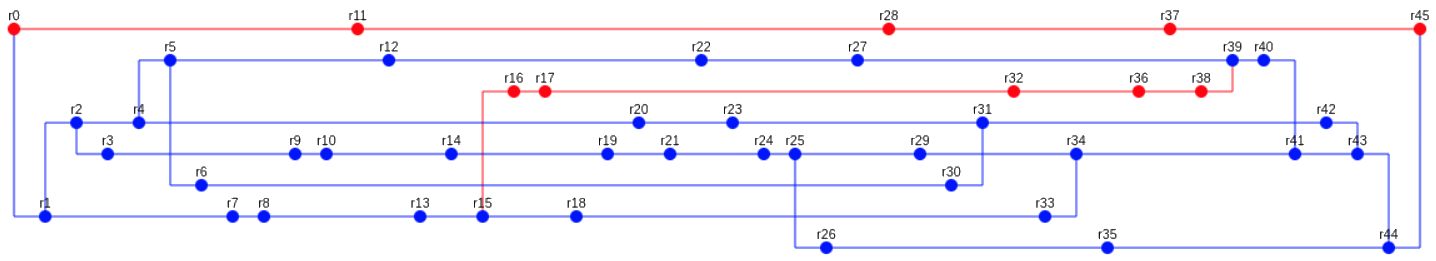
\includegraphics[scale=1.3]{img/scheme}
\end{figure}

\section{SVN:}
\subsection{Конфигурация репозитория:}
\tiny
\begin{verbatim}
svnadmin create repo
cd repo
svn mkdir -m "create structure" file:///home/studs/s336759/repo/trunk file:///home/studs/s336759/repo/branches file:///home/studs/s336759/repo/tags --username="DoraGotova"
svn checkout file:///home/studs/s336759/repo/trunk workspace
cd workspace
\end{verbatim}
\normalsize
\subsection{Список команд:}
%! Author = kyoto
%! Date = 18.04.2023

\tiny
\begin{verbatim}
# r0
mv -f ~/src/commit0/* ./
svn add *
svn commit -m "commit r0" --username "DoraGotova"

# r1
svn copy file:///home/studs/s336759/repo/trunk file:///home/studs/s336759/repo/branches/fork_from_r0 -m "forked from r0" --username="DEAD_INSIDE_PSYCHOGHOUL_KANEKI_KEN_GENEI_RYODAN_4_1000-7"
svn switch file:///home/studs/s336759/repo/branches/fork_from_r0
mv -f ~/src/commit1/* ./
svn add *
svn commit -m "commit r1" --username="DEAD_INSIDE_PSYCHOGHOUL_KANEKI_KEN_GENEI_RYODAN_4_1000-7"


# r2
svn copy file:///home/studs/s336759/repo/branches/fork_from_r0 file:///home/studs/s336759/repo/branches/fork_from_r1 -m "forked from r1" --username="DEAD_INSIDE_PSYCHOGHOUL_KANEKI_KEN_GENEI_RYODAN_4_1000-7"
svn switch file:///home/studs/s336759/repo/branches/fork_from_r1
mv -f ~/src/commit2/* ./
svn add *
svn commit -m "commit r2" --username="DEAD_INSIDE_PSYCHOGHOUL_KANEKI_KEN_GENEI_RYODAN_4_1000-7"

# r3
svn copy file:///home/studs/s336759/repo/branches/fork_from_r1 file:///home/studs/s336759/repo/branches/fork_from_r2 -m "forked from r2" --username="DEAD_INSIDE_PSYCHOGHOUL_KANEKI_KEN_GENEI_RYODAN_4_1000-7"
svn switch file:///home/studs/s336759/repo/branches/fork_from_r2
mv -f ~/src/commit3/* ./
svn add *
svn commit -m "commit r3" --username="DEAD_INSIDE_PSYCHOGHOUL_KANEKI_KEN_GENEI_RYODAN_4_1000-7"

# r4
svn switch file:///home/studs/s336759/repo/branches/fork_from_r1
mv -f ~/src/commit4/* ./
svn add *
svn commit -m "commit r4" --username="DEAD_INSIDE_PSYCHOGHOUL_KANEKI_KEN_GENEI_RYODAN_4_1000-7"

# r5
svn copy file:///home/studs/s336759/repo/branches/fork_from_r1 file:///home/studs/s336759/repo/branches/fork_from_r4 -m "forked from r4" --username="DEAD_INSIDE_PSYCHOGHOUL_KANEKI_KEN_GENEI_RYODAN_4_1000-7"
svn switch file:///home/studs/s336759/repo/branches/fork_from_r4
mv -f ~/src/commit5/* ./
svn add *
svn commit -m "commit r5" --username="DEAD_INSIDE_PSYCHOGHOUL_KANEKI_KEN_GENEI_RYODAN_4_1000-7"

# r6
svn copy file:///home/studs/s336759/repo/branches/fork_from_r4 file:///home/studs/s336759/repo/branches/fork_from_r5 -m "forked from r5" --username="DEAD_INSIDE_PSYCHOGHOUL_KANEKI_KEN_GENEI_RYODAN_4_1000-7"
svn switch file:///home/studs/s336759/repo/branches/fork_from_r5
mv -f ~/src/commit6/* ./
svn add *
svn commit -m "commit r6" --username="DEAD_INSIDE_PSYCHOGHOUL_KANEKI_KEN_GENEI_RYODAN_4_1000-7"

# r7
svn switch file:///home/studs/s336759/repo/branches/fork_from_r0
mv -f ~/src/commit7/* ./
svn add *
svn commit -m "commit r7" --username="DEAD_INSIDE_PSYCHOGHOUL_KANEKI_KEN_GENEI_RYODAN_4_1000-7"

# r8
mv -f ~/src/commit8/* ./
svn add *
svn commit -m "commit r8" --username="DEAD_INSIDE_PSYCHOGHOUL_KANEKI_KEN_GENEI_RYODAN_4_1000-7"

# r9
svn switch file:///home/studs/s336759/repo/branches/fork_from_r2
mv -f ~/src/commit9/* ./
svn add *
svn commit -m "commit r9" --username="DEAD_INSIDE_PSYCHOGHOUL_KANEKI_KEN_GENEI_RYODAN_4_1000-7"

# r10
mv -f ~/src/commit10/* ./
svn add *
svn commit -m "commit r10" --username="DEAD_INSIDE_PSYCHOGHOUL_KANEKI_KEN_GENEI_RYODAN_4_1000-7"

# r11
svn switch file:///home/studs/s336759/repo/trunk
mv -f ~/src/commit11/* ./
svn add *
svn commit -m "commit r11" --username="DoraGotova"

# r12
svn switch file:///home/studs/s336759/repo/branches/fork_from_r4
mv -f ~/src/commit12/* ./
svn add *
svn commit -m "commit r12" --username="DEAD_INSIDE_PSYCHOGHOUL_KANEKI_KEN_GENEI_RYODAN_4_1000-7"

# r13
svn switch file:///home/studs/s336759/repo/branches/fork_from_r0
mv -f ~/src/commit13/* ./
svn add *
svn commit -m "commit r13" --username="DEAD_INSIDE_PSYCHOGHOUL_KANEKI_KEN_GENEI_RYODAN_4_1000-7"

# r14
svn switch file:///home/studs/s336759/repo/branches/fork_from_r2
mv -f ~/src/commit14/* ./
svn add *
svn commit -m "commit r14" --username="DEAD_INSIDE_PSYCHOGHOUL_KANEKI_KEN_GENEI_RYODAN_4_1000-7"

# r15
svn switch file:///home/studs/s336759/repo/branches/fork_from_r0
mv -f ~/src/commit15/* ./
svn add *
svn commit -m "commit r15" --username="DEAD_INSIDE_PSYCHOGHOUL_KANEKI_KEN_GENEI_RYODAN_4_1000-7"

# r16
svn copy file:///home/studs/s336759/repo/branches/fork_from_r0 file:///home/studs/s336759/repo/branches/fork_from_r15 -m "forked from r15" --username="DoraGotova"
svn switch file:///home/studs/s336759/repo/branches/fork_from_r15
mv -f ~/src/commit16/* ./
svn add *
svn commit -m "commit r16" --username="DoraGotova"

# r17
mv -f ~/src/commit17/* ./
svn add *
svn commit -m "commit r17" --username="DoraGotova"

# r18
svn switch file:///home/studs/s336759/repo/branches/fork_from_r0
mv -f ~/src/commit18/* ./
svn add *
svn commit -m "commit r18" --username="DEAD_INSIDE_PSYCHOGHOUL_KANEKI_KEN_GENEI_RYODAN_4_1000-7"

# r19
svn switch file:///home/studs/s336759/repo/branches/fork_from_r2
mv -f ~/src/commit19/* ./
svn add *
svn commit -m "commit r19" --username="DEAD_INSIDE_PSYCHOGHOUL_KANEKI_KEN_GENEI_RYODAN_4_1000-7"

# r20
svn switch file:///home/studs/s336759/repo/branches/fork_from_r1
mv -f ~/src/commit20/* ./
svn add *
svn commit -m "commit r20" --username="DEAD_INSIDE_PSYCHOGHOUL_KANEKI_KEN_GENEI_RYODAN_4_1000-7"

# r21
svn switch file:///home/studs/s336759/repo/branches/fork_from_r2
mv -f ~/src/commit21/* ./
svn add *
svn commit -m "commit r21" --username="DEAD_INSIDE_PSYCHOGHOUL_KANEKI_KEN_GENEI_RYODAN_4_1000-7"

# r22
svn switch file:///home/studs/s336759/repo/branches/fork_from_r4
mv -f ~/src/commit22/* ./
svn add *
svn commit -m "commit r22" --username="DEAD_INSIDE_PSYCHOGHOUL_KANEKI_KEN_GENEI_RYODAN_4_1000-7"

# r23
svn switch file:///home/studs/s336759/repo/branches/fork_from_r1
mv -f ~/src/commit23/* ./
svn add *
svn commit -m "commit r23" --username="DEAD_INSIDE_PSYCHOGHOUL_KANEKI_KEN_GENEI_RYODAN_4_1000-7"

# r24
svn switch file:///home/studs/s336759/repo/branches/fork_from_r2
mv -f ~/src/commit24/* ./
svn add *
svn commit -m "commit r24" --username="DEAD_INSIDE_PSYCHOGHOUL_KANEKI_KEN_GENEI_RYODAN_4_1000-7"

# r25
mv -f ~/src/commit25/* ./
svn add *
svn commit -m "commit r25" --username="DEAD_INSIDE_PSYCHOGHOUL_KANEKI_KEN_GENEI_RYODAN_4_1000-7"

# r26
svn copy file:///home/studs/s336759/repo/branches/fork_from_r2 file:///home/studs/s336759/repo/branches/fork_from_r25 -m "forked from r25" --username="DEAD_INSIDE_PSYCHOGHOUL_KANEKI_KEN_GENEI_RYODAN_4_1000-7"
svn switch file:///home/studs/s336759/repo/branches/fork_from_r25
mv -f ~/src/commit26/* ./
svn add *
svn commit -m "commit r26" --username="DEAD_INSIDE_PSYCHOGHOUL_KANEKI_KEN_GENEI_RYODAN_4_1000-7"

# r27
svn switch file:///home/studs/s336759/repo/branches/fork_from_r4
mv -f ~/src/commit27/* ./
svn add *
svn commit -m "commit r27" --username="DEAD_INSIDE_PSYCHOGHOUL_KANEKI_KEN_GENEI_RYODAN_4_1000-7"

# r28
svn switch file:///home/studs/s336759/repo/trunk
mv -f ~/src/commit28/* ./
svn add *
svn commit -m "commit r28" --username="DoraGotova"

# r29
svn switch file:///home/studs/s336759/repo/branches/fork_from_r2
mv -f ~/src/commit29/* ./
svn add *
svn commit -m "commit r29" --username="DEAD_INSIDE_PSYCHOGHOUL_KANEKI_KEN_GENEI_RYODAN_4_1000-7"

# r30
svn switch file:///home/studs/s336759/repo/branches/fork_from_r5
mv -f ~/src/commit30/* ./
svn add *
svn commit -m "commit r30" --username="DEAD_INSIDE_PSYCHOGHOUL_KANEKI_KEN_GENEI_RYODAN_4_1000-7"

# r31
svn switch file:///home/studs/s336759/repo/branches/fork_from_r1
svn merge file:///home/studs/s336759/repo/branches/fork_from_r5 file:///home/studs/s336759/repo/branches/fork_from_r1 --username="DEAD_INSIDE_PSYCHOGHOUL_KANEKI_KEN_GENEI_RYODAN_4_1000-7"
svn commit -m "merge r30 into r31" --username="DEAD_INSIDE_PSYCHOGHOUL_KANEKI_KEN_GENEI_RYODAN_4_1000-7"
mv -f ~/src/commit31/* ./
svn add *
svn commit -m "commit r31" --username="DEAD_INSIDE_PSYCHOGHOUL_KANEKI_KEN_GENEI_RYODAN_4_1000-7"

# r32
svn switch file:///home/studs/s336759/repo/branches/fork_from_r15
mv -f ~/src/commit32/* ./
svn add *
svn commit -m "commit r32" --username="DoraGotova"

# r33
svn switch file:///home/studs/s336759/repo/branches/fork_from_r0
mv -f ~/src/commit33/* ./
svn add *
svn commit -m "commit r33" --username="DEAD_INSIDE_PSYCHOGHOUL_KANEKI_KEN_GENEI_RYODAN_4_1000-7"

# r34
svn switch file:///home/studs/s336759/repo/branches/fork_from_r2
svn merge file:///home/studs/s336759/repo/branches/fork_from_r0 file:///home/studs/s336759/repo/branches/fork_from_r2 --username="DEAD_INSIDE_PSYCHOGHOUL_KANEKI_KEN_GENEI_RYODAN_4_1000-7"
mv -f ~/src/commit34/* ./
svn add *
svn commit -m "commit r34" --username="DEAD_INSIDE_PSYCHOGHOUL_KANEKI_KEN_GENEI_RYODAN_4_1000-7"

# r35
svn switch file:///home/studs/s336759/repo/branches/fork_from_r25
mv -f ~/src/commit35/* ./
svn add *
svn commit -m "commit r35" --username="DEAD_INSIDE_PSYCHOGHOUL_KANEKI_KEN_GENEI_RYODAN_4_1000-7"

# r36
svn switch file:///home/studs/s336759/repo/branches/fork_from_r15
mv -f ~/src/commit36/* ./
svn add *
svn commit -m "commit r36" --username="DoraGotova"

# r37
svn switch file:///home/studs/s336759/repo/trunk
mv -f ~/src/commit37/* ./
svn add *
svn commit -m "commit r37" --username="DoraGotova"

# r38
svn switch file:///home/studs/s336759/repo/branches/fork_from_r15
mv -f ~/src/commit38/* ./
svn add *
svn commit -m "commit r38" --username="DoraGotova"

# r39 -conflict i
svn switch file:///home/studs/s336759/repo/branches/fork_from_r4
svn merge file:///home/studs/s336759/repo/branches/fork_from_r15 file:///home/studs/s336759/repo/branches/fork_from_r4 --username="DoraGotova"
svn commit -m "merge r38 into r39" --username="DoraGotova"
mv -f ~/src/commit39/* ./
svn add *
svn commit -m "commit r39" --username="DEAD_INSIDE_PSYCHOGHOUL_KANEKI_KEN_GENEI_RYODAN_4_1000-7"

# r40
mv -f ~/src/commit40/* ./
svn add *
svn commit -m "commit r40" --username="DEAD_INSIDE_PSYCHOGHOUL_KANEKI_KEN_GENEI_RYODAN_4_1000-7"

# r41 - 2 conflicts m,m
svn switch file:///home/studs/s336759/repo/branches/fork_from_r2
svn merge file:///home/studs/s336759/repo/branches/fork_from_r4 file:///home/studs/s336759/repo/branches/fork_from_r2 --username="DEAD_INSIDE_PSYCHOGHOUL_KANEKI_KEN_GENEI_RYODAN_4_1000-7"
svn commit -m "merge r40 into r41" --username="DEAD_INSIDE_PSYCHOGHOUL_KANEKI_KEN_GENEI_RYODAN_4_1000-7"
mv -f ~/src/commit41/* ./
svn add *
svn commit -m "commit r41" --username="DEAD_INSIDE_PSYCHOGHOUL_KANEKI_KEN_GENEI_RYODAN_4_1000-7"

# r42
svn switch file:///home/studs/s336759/repo/branches/fork_from_r1
mv -f ~/src/commit42/* ./
svn add *
svn commit -m "commit r42" --username="DEAD_INSIDE_PSYCHOGHOUL_KANEKI_KEN_GENEI_RYODAN_4_1000-7"

# r43 - 3 cinflicts m,m,m
svn switch file:///home/studs/s336759/repo/branches/fork_from_r2
svn merge file:///home/studs/s336759/repo/branches/fork_from_r1 file:///home/studs/s336759/repo/branches/fork_from_r2 --username="DEAD_INSIDE_PSYCHOGHOUL_KANEKI_KEN_GENEI_RYODAN_4_1000-7"
svn commit -m "merge r42 into r43" --username="DEAD_INSIDE_PSYCHOGHOUL_KANEKI_KEN_GENEI_RYODAN_4_1000-7"
mv -f ~/src/commit43/* ./
svn add *
svn commit -m "commit r43" --username="DEAD_INSIDE_PSYCHOGHOUL_KANEKI_KEN_GENEI_RYODAN_4_1000-7"

# r44 -conflict i
svn switch file:///home/studs/s336759/repo/branches/fork_from_r25
svn merge file:///home/studs/s336759/repo/branches/fork_from_r2 file:///home/studs/s336759/repo/branches/fork_from_r25 --username="DEAD_INSIDE_PSYCHOGHOUL_KANEKI_KEN_GENEI_RYODAN_4_1000-7"
svn commit -m "merge r43 into r44" --username="DEAD_INSIDE_PSYCHOGHOUL_KANEKI_KEN_GENEI_RYODAN_4_1000-7"
mv -f ~/src/commit44/* ./
svn add *
svn commit -m "commit r44" --username="DEAD_INSIDE_PSYCHOGHOUL_KANEKI_KEN_GENEI_RYODAN_4_1000-7"

# r45 - 4 conflicts
svn switch file:///home/studs/s336759/repo/trunk
svn merge file:///home/studs/s336759/repo/branches/fork_from_r25 file:///home/studs/s336759/repo/trunk --username="DEAD_INSIDE_PSYCHOGHOUL_KANEKI_KEN_GENEI_RYODAN_4_1000-7"
svn commit -m "merge r44 into r45" --username="DEAD_INSIDE_PSYCHOGHOUL_KANEKI_KEN_GENEI_RYODAN_4_1000-7"
mv -f ~/src/commit45/* ./
svn add *
svn commit -m "commit r45" --username="DoraGotova"
\end{verbatim}
\normalsize
\section{GIT:}
\subsection{Конфигурация репозитория:}
%! Author = kyoto
%! Date = 18.04.2023

\tiny
\begin{verbatim}
git init gitrepo
cd gitrepo
\end{verbatim}
\normalsize
\subsection{Список команд:}
%! Author = kyoto
%! Date = 18.04.2023

\tiny
\begin{verbatim}
# r0
git config --global user.name "DoraGotova"
git config --global user.email "DoraGotova@gmail.com"
mv -f ~/src/commit0/* ./
git add *
git commit -m "commit r0"

# r1
git config --global user.name "maybemaybebaby"
git config --global user.email "maybemaybebay@gmail.com"
git checkout -b fork_from_r0
mv -f ~/src/commit1/* ./
git add *
git commit -m "commit r1"

# r2
git checkout -b fork_from_r1
mv -f ~/src/commit2/* ./
git add *
git commit -m "commit r2"

# r3
git checkout -b fork_from_r2
mv -f ~/src/commit3/* ./
git add *
git commit -m "commit r3"

# r4
git checkout fork_from_r1
mv -f ~/src/commit4/* ./
git add &
git commit -m "commit r4"

# r5
git checkout -b fork_from_r4
mv -f ~/src/commit5/* ./
git add *
git commit -m "commit r5"

# r6
git checkout -b fork_from_r5
mv -f ~/src/commit6/* ./
git add *
git commit -m "commit r6"

# r7
git checkout fork_from_r0
mv -f ~/src/commit7/* ./
git add *
git commit -m "commit r7"

# r8
mv -f ~/src/commit8/* ./
git add *
git commit -m "commit r8"

# r9
git checkout fork_from_r2
mv -f ~/src/commit9/* ./
git add *
git commit -m "commit r9"

# r10
mv -f ~/src/commit10/* ./
git add *
git commit -m "commit r10"

# r11
git config --global user.name "DoraGotova"
git config --global user.email "DoraGotova@gmail.com"
git checkout master
mv -f ~/src/commit11/* ./
git add *
git commit -m "commit r11"

# r12
git config --global user.name "maybemaybebaby"
git config --global user.email "maybemaybebay@gmail.com"
git checkout fork_from_r4
mv -f ~/src/commit12/* ./
git add *
git commit -m "commit r12"

# r13
git checkout fork_from_r0
mv -f ~/src/commit13/* ./
git add *
git commit -m "commit r13"

# r14
git checkout fork_from_r2
mv -f ~/src/commit14/* ./
git add *
git commit -m "commit r14"

# r15
git checkout fork_from_r0
mv -f ~/src/commit15/* ./
git add *
git commit -m "commit r15"

# r16
git config --global user.name "DoraGotova"
git config --global user.email "DoraGotova@gmail.com"
git checkout -b fork_from_r15
mv -f ~/src/commit16/* ./
git add *
git commit -m "commit r16"

# r17
mv -f ~/src/commit17/* ./
git add *
git commit -m "commit r17"

# r18
git config --global user.name "maybemaybebaby"
git config --global user.email "maybemaybebay@gmail.com"
git checkout fork_from_r0
mv -f ~/src/commit18/* ./
git add *
git commit -m "commit r18"

# r19
git checkout fork_from_r2
mv -f ~/src/commit19/* ./
git add *
git commit -m "commit r19"

# r20
git checkout fork_from_r1
mv -f ~/src/commit20/* ./
git add *
git commit -m "commit r20"

# r21
git checkout fork_from_r2
mv -f ~/src/commit21/* ./
git add *
git commit -m "commit r21"

# r22
git checkout fork_from_r4
mv -f ~/src/commit22/* ./
git add *
git commit -m "commit r22"

# r23
git checkout fork_from_r1
mv -f ~/src/commit23/* ./
git add *
git commit -m "commit r23"

# r24
git checkout fork_from_r2
mv -f ~/src/commit24/* ./
git add *
git commit -m "commit r24"

# r25
mv -f ~/src/commit25/* ./
git add *
git commit -m "commit r25"
git checkout -b fork_from_r25

# r26
mv -f ~/src/commit26/* ./
git add *
git commit -m "commit r26"

# r27
git checkout fork_from_r4
mv -f ~/src/commit27/* ./
git add *
git commit -m "commit r27"

# r28
git config --global user.name "DoraGotova"
git config --global user.email "DoraGotova@gmail.com"
git checkout master
mv -f ~/src/commit28/* ./
git add *
git commit -m "commit r28"

# r29
git config --global user.name "maybemaybebaby"
git config --global user.email "maybemaybebay@gmail.com"
git checkout fork_from_r2
mv -f ~/src/commit29/* ./
git add *
git commit -m "commit r29"

# r30
git checkout fork_from_r5
mv -f ~/src/commit30/* ./
git add *
git commit -m "commit r30"

# r31
git checkout fork_from_r1
git merge fork_from_r5 -m "merge r30 into r31"
mv -f ~/src/commit31/* ./
git add *
git commit -m "commit r31"

# r32
git config --global user.name "DoraGotova"
git config --global user.email "DoraGotova@gmail.com"
git checkout fork_from_r15
mv -f ~/src/commit32/* ./
git add *
git commit -m "commit r32"

# r33
git config --global user.name "maybemaybebaby"
git config --global user.email "maybemaybebay@gmail.com"
git checkout fork_from_r0
mv -f ~/src/commit33/* ./
git add *
git commit -m "commit r33"

# r34
git checkout fork_from_r2
git merge fork_from_r0 -m "merge r33 into r34"
\end{verbatim}
\normalsize
\textit{resolving conflicts...}
%! Author = kyoto
%! Date = 18.04.2023

\tiny
\begin{verbatim}
git add *
git commit -m "merge r33 into r34"
mv -f ~/src/commit34/* ./
git add *
git commit -m "commit r34"

# r35
git checkout fork_from_r25
mv -f ~/src/commit35/* ./
git add *
git commit -m "commit r35"

# r36
git config --global user.name "DoraGotova"
git config --global user.email "DoraGotova@gmail.com"
git checkout fork_from_r15
mv -f ~/src/commit36/* ./
git add *
git commit -m "commit r36"

# r37
git checkout master
mv -f ~/src/commit37/* ./
git add *
git commit -m "commit r37"

# r38
git checkout fork_from_r15
mv -f ~/src/commit38/* ./
git add *
git commit -m "commit r38"

# r39 - conflict
git checkout fork_from_r4
git merge fork_from_r15 -m "merge r38 into r39"


\end{verbatim}
\normalsize
\textit{resolving conflicts...}
%! Author = kyoto
%! Date = 18.04.2023

\tiny
\begin{verbatim}
git add *
git commit -m "merge r38 into r39"
git config --global user.name "maybemaybebaby"
git config --global user.email "maybemaybebay@gmail.com"
mv -f ~/src/commit39/* ./
git add *
git commit -m "commit r39"

# r40
mv -f ~/src/commit40/* ./
git add *
git commit -m "commit r40"

# r41
git checkout fork_from_r2
git merge fork_from_r4 -m "merge r40 into r41"

\end{verbatim}
\normalsize
\newpage

\thispagestyle{empty}
\BgThispage


\textit{resolving conflicts...}
%! Author = kyoto
%! Date = 18.04.2023

\tiny
\begin{verbatim}
git add *
git commit -m "merge r40 into r41"
mv -f ~/src/commit41/* ./
git add *
git commit -m "commit r41"

# r42
git checkout fork_from_r1
mv -f ~/src/commit42/* ./
git add *
git commit -m "commit r42"

# r43
git checkout fork_from_r2
git merge fork_from_r1 -m "merge r42 into r43"
\end{verbatim}
\normalsize
\textit{resolving conflicts...}
%! Author = kyoto
%! Date = 18.04.2023

\tiny
\begin{verbatim}
git add *
git commit -m "merge r42 into r43"
mv -f ~/src/commit43/* ./
git add *
git commit -m "commit r43"

# r44
git checkout fork_from_r25
git merge fork_from_r2 -m "merge r43 into r44"

\end{verbatim}
\normalsize
\textit{resolving conflicts...}
%! Author = kyoto
%! Date = 18.04.2023

\tiny
\begin{verbatim}
git add *
git commit -m "merge r43 itno r44"
mv -f ~/src/commit44/* ./
git add *
git commit -m "commit r44"

# r45
git checkout master
git merge fork_from_r25 -m "merge r44 into r45"
\end{verbatim}
\normalsize
\textit{resolving conflicts...}
%! Author = kyoto
%! Date = 18.04.2023

\tiny
\begin{verbatim}
git add *
git commit -m "merge r44 itno r45"
git config --global user.name "DoraGotova"
git config --global user.email "DoraGotova@gmail.com"
mv -f ~/src/commit45/* ./
git add *
git commit -m "commit r45"
\end{verbatim}
\normalsize

\section{Выводы:}
ахуенная лаба братанчик пасиба
